\documentclass[conference]{IEEEtran}
\usepackage[T1]{fontenc}
\usepackage{mathptmx}
\usepackage{balance}
\usepackage{amsmath,amssymb,graphicx,booktabs,url}
\usepackage[hidelinks]{hyperref}
\graphicspath{{../artifacts/figures/}}
\begin{document}
\title{Traffic Sign Recognition Under Image Degradation:\\A Controlled Comparison of HOG--SVM and CNNs}
\author{}
\maketitle
\begin{abstract}
Traffic sign recognition can perform well on familiar images while remaining sensitive to reduced image quality. This project compares a histogram-of-oriented-gradients (HOG) linear support vector machine, a compact convolutional neural network (CNN), and an identical CNN trained with corruption augmentation on the German Traffic Sign Recognition Benchmark. All models use the same track-disjoint training and validation split, and are evaluated on the complete official test set of 12,630 images. Gaussian blur, reduced brightness, and additive Gaussian noise are applied at three severities after resizing. Clean test accuracies are 77.55\%, 98.38\%, and 97.33\%, respectively. Mean accuracy across the nine corrupted conditions is 55.55\%, 88.18\%, and 94.47\%. Augmentation changes mean corrupted accuracy by +6.29 percentage points relative to the clean-trained CNN. These measurements characterize a controlled synthetic-corruption study; they do not establish performance in a full driving system. Source code, trained weights, predictions, and reproducibility records accompany this report.
\end{abstract}
\begin{IEEEkeywords}
traffic sign recognition, HOG, support vector machine, convolutional neural network, corruption robustness
\end{IEEEkeywords}

\section{Introduction}
Recognizing a traffic sign requires distinguishing categories whose appearance may differ only in a digit, a symbol, or a local arrangement of edges. Image blur can erase those details, reduced brightness can suppress contrast, and noise can introduce misleading gradients. A classifier's accuracy on the original test images therefore answers only part of the recognition problem. A useful complementary question is how its predictions change when a controlled transformation reduces the information in those images.

This project studies that question using the German Traffic Sign Recognition Benchmark (GTSRB)~\cite{gtsrb}. The scope is single-image classification of already cropped signs into 43 categories. Detecting signs in street scenes, tracking across video frames, and interpreting road context are outside the experiment. Keeping the scope narrow makes it possible to examine representation, training conditions, and image quality with a shared data pipeline.

The first comparison is between engineered gradient features followed by a linear classifier and features learned by a CNN. The second is a controlled training intervention: the two CNNs have the same architecture, initialization seed, optimizer, epoch budget, and validation criterion, while one receives randomly corrupted training images. The research question is whether this intervention improves recognition under the selected distortions, and what it costs on the original test distribution.

The project contributes (1) a reproducible comparison using a split that separates sign tracks rather than individual frames; (2) evaluation on ten conditions, comprising the original test set and nine synthetic corruptions; and (3) quantitative and qualitative analysis using accuracy, macro F1, per-class results, confusion matrices, and paired prediction outcomes. The contribution is an experimental implementation and analysis, not a new network architecture or a claim of state-of-the-art performance.

\subsection{Related Work}
Stallkamp \emph{et al.} introduced a traffic-sign benchmark with substantial within-class appearance variation and compared recognition methods~\cite{gtsrb}. GTSRB contains sequences of views of individual physical signs. Keeping such views together in the training/validation partition avoids assessing the model on highly related views of a sign already used for fitting. The official test partition is retained without modification in this project.

HOG describes an image using locally normalized orientation histograms~\cite{hog}. Although originally demonstrated for human detection, its representation supplies a useful classical baseline for a shape-dependent recognition task. The implementation here uses a compact descriptor and a linear SVM; it is not a reproduction of the original HOG detector. CNNs instead optimize convolutional filters jointly with the classifier. The clean and augmented variants allow a direct comparison of training distributions without introducing transfer learning as an additional variable.

Hendrycks and Dietterich emphasize measuring recognition under common image corruptions~\cite{corruption}. The present study follows the principle of evaluating multiple controlled conditions, but its dataset, transformation settings, number of severities, and aggregate metric are project-specific. The reported mean corrupted accuracy is not ImageNet-C's normalized mean corruption error, and the results should not be compared numerically with that benchmark.

AugMix~\cite{augmix} is a representative augmentation-based robustness method that mixes transformed images and encourages prediction consistency. The intervention studied here is simpler: one selected degradation is applied per image, with ordinary supervised cross-entropy and no consistency objective. Consequently, the augmented CNN should not be described as an implementation of AugMix. Comparing these strategies would be a useful extension once the basic effects are established.

Recent visual representation learning also includes large self-supervised foundation models. DINOv3~\cite{dinov3}, released in 2025, scales visual pretraining and introduces Gram anchoring to maintain dense-feature quality during long training. Such pretrained features provide a broader contemporary alternative to training a small CNN from scratch. They are not evaluated here: introducing large external pretraining would change the data and compute assumptions of the controlled comparison. The present report situates its compact baselines within that wider literature without claiming parity with foundation-model performance.

\section{Technical Approach}
\begin{figure*}[t]
\centering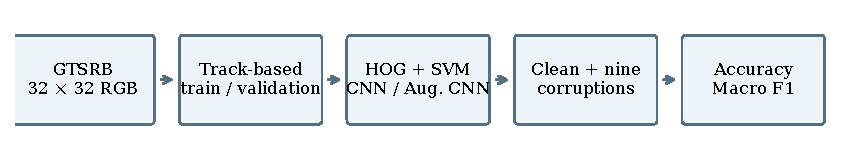
\includegraphics[width=.98\textwidth]{pipeline.pdf}
\caption{Shared experimental pipeline. Model fitting and checkpoint selection use only the training and validation partitions. The official test set supplies the ten final evaluation conditions.}
\label{fig:pipeline}
\end{figure*}
\subsection{Input Representation and Data Integrity}
All input images are converted to three-channel RGB and resized to $32\times32$ pixels using bilinear interpolation. CNN inputs are scaled to $[0,1]$. Images are treated as full sign crops; the bounding-box metadata is not used for a second crop. This choice preserves surrounding information consistently for all three models and avoids introducing a different crop policy in the demo.

The local CSV files contain absolute-looking paths beginning with \texttt{/code/}. The loader removes that known prefix and resolves the remaining path relative to the dataset root. Paths that would escape the root are rejected. Each CSV row supplies the class identifier and image path; the 43 class names come from the supplied label file. This makes the implementation independent of the original download location while preserving the dataset's existing labels.

\subsection{HOG and Linear SVM}
RGB images are converted to grayscale before HOG extraction. The descriptor uses nine orientation bins, $8\times8$-pixel cells, and $2\times2$-cell blocks with L2-Hys normalization. A $32\times32$ image has $4\times4$ cells and $3\times3$ overlapping blocks, giving
\begin{equation}
d=3\cdot3\cdot2\cdot2\cdot9=324
\end{equation}
features. Training-set feature means and scales are fitted by a standardizer. The same fitted transform is then applied to validation, test, and demo inputs.

A one-versus-rest linear SVM uses $C=1$, squared hinge loss, and a maximum of 10,000 optimization iterations. Conceptually, each binary classifier balances a weight penalty against margin violations:
\begin{equation}
\min_{w,b}\ \tfrac12\lVert w\rVert_2^2+C\sum_i\max(0,1-y_i(w^\top z_i+b))^2.
\end{equation}
The baseline deliberately uses a linear decision function. Its performance measures this particular compact representation and classifier; a gap relative to a CNN is not evidence that every feature-based or kernel method would have the same gap. The selected $C$ is fixed in advance, without a test-set parameter search.

\subsection{Compact CNN}
The CNN has three convolutional blocks with 32, 64, and 128 output channels. Each block contains two $3\times3$ convolutions with padding one, each followed by batch normalization and ReLU, then $2\times2$ max pooling. Spatial resolution changes from $32$ to $16$, $8$, and $4$. The resulting $128\times4\times4$ feature map is flattened into a 256-unit fully connected layer, ReLU, dropout with probability 0.3, and a 43-logit output layer. The model contains 823,499 trainable parameters.

For logits $s$ and class label $y$, the training objective is multiclass cross-entropy,
\begin{equation}
\mathcal{L}(s,y)=-\log\frac{\exp s_y}{\sum_{c=0}^{42}\exp s_c}.
\end{equation}
Both CNNs use AdamW~\cite{adamw}, learning rate $10^{-3}$, weight decay $10^{-4}$, batch size 256, and 24 epochs. Cosine scheduling decreases the learning rate toward $10^{-5}$. The checkpoint with highest clean validation macro F1 is retained. The two networks start from the same seeded initialization; stochastic operations during augmentation can cause their subsequent random-number sequences to differ.

\subsection{Corruption Augmentation}
For each training image presented to the augmented CNN, one of four outcomes is selected with equal probability: unchanged input, blur, darkness, or noise. Darkness multiplies all channels by a random factor in $[0.2,0.9)$. Noise adds independent zero-mean Gaussian values with a standard deviation sampled from $[0.02,0.14)$ in the normalized scale. Values are clipped to $[0,1]$.

Training blur is implemented as separable Gaussian convolution with replicated boundaries and a 13-tap kernel. A standard deviation in $[0.4,1.8)$ is sampled for each batch's blurred subset. Final evaluation uses Pillow's Gaussian-blur implementation. These implement the same family of degradation with different discrete approximations; they are not assumed pixel-identical. No image flips, rotations, external images, or pretrained weights are used. The intervention is therefore limited to exposure to image-quality distortions.

\section{Experimental Setup}
\subsection{Dataset and Track-Disjoint Split}
The provided GTSRB copy contains 39,209 training-partition images and 12,630 official test images, covering all 43 classes. A training filename encodes class, sign track, and frame. For each class separately, the implementation deterministically shuffles its unique tracks using seed 42, assigns approximately 20\% of tracks to validation, and keeps the remainder for fitting. All frames of a track follow that track's assignment. Rounding occurs at track level rather than image level.

The realized partition contains 31,380 fitting images in 1,046 tracks and 7,829 validation images in 261 tracks. All 43 categories occur in both partitions, and their track intersection is empty. The official test set is never used for gradient updates, standardizer fitting, or checkpoint selection. Split membership is exported row by row, and input CSV hashes are saved in the experiment manifest. These checks establish consistency with the provided dataset copy; they do not independently authenticate every original image against an upstream checksum.

\subsection{Evaluation Conditions}
Each official test image is first resized, then transformed independently. Table~\ref{tab:conditions} defines the nine corrupted conditions. For blur, the parameter is the Gaussian radius in the resized image's pixel units. For darkness, it is the multiplicative brightness factor. For noise, it is the standard deviation relative to $[0,1]$ intensities. Clipping and conversion back to unsigned 8-bit RGB follow the transformation. Noise uses a deterministic seed of $42+i$ for test image $i$, so every model receives identical corrupted images.

\begin{table}[t]\centering
\caption{Project-specific corruption parameters. Severity 0 is the unchanged image for every transformation.}\label{tab:conditions}
\begin{tabular}{lccc}\toprule
Transformation & Level 1 & Level 2 & Level 3\\\midrule
Gaussian blur radius & 0.6 & 1.2 & 1.8\\
Brightness multiplier & 0.65 & 0.40 & 0.20\\
Gaussian noise std. & 0.04 & 0.08 & 0.12\\\bottomrule
\end{tabular}\end{table}

The original test images themselves already exhibit natural variation. Thus, ``clean'' means the unchanged official image after shared preprocessing, rather than a guarantee of perfect lighting or focus. Synthetic darkness scales pixel intensities directly; it does not simulate camera exposure, sensor behavior, glare, or nighttime scene geometry. Similarly, Gaussian blur is not a full motion-blur model.

\subsection{Metrics and Comparison Policy}
Accuracy is the fraction of correctly classified images. Macro F1 averages class-wise F1 across all 43 categories, giving each category equal weight regardless of its support:
\begin{equation}
F_{1,\mathrm{macro}}=\frac1{43}\sum_{c=0}^{42}\frac{2P_cR_c}{P_c+R_c}.
\end{equation}
An undefined class-wise score is set to zero. The aggregate corrupted accuracy is an equally weighted average over the nine conditions:
\begin{equation}
A_{\mathrm{corr}}=\frac19\sum_{k=1}^{3}\sum_{s=1}^{3}A_{k,s}.
\end{equation}
This weighting is a reporting choice, not an estimate of how frequently these distortions occur on a road. Conditions reuse the same source images and should not be interpreted as nine independent datasets.

All settings are shared or fixed as stated, with one random seed and one training run per CNN. No significance claim is made from that single run. Model comparisons describe the measured checkpoints; variation across seeds and alternative hyperparameters remains unmeasured. Paired severe-condition counts additionally show when the two CNNs succeed on the same image and when only one is correct.

\subsection{Implementation and Compute}
The experiment ran on an NVIDIA GeForce RTX 4060 Ti with 16 GB of GPU memory, using Python 3.12.10, PyTorch 2.8.0+cu128, and scikit-learn 1.7.2. CNN weights and SVM preprocessing are saved together with the experiment outputs. Recorded fitting times were 145.3 seconds for HOG extraction and SVM fitting, 243.2 seconds for the clean CNN, and 262.2 seconds for the augmented CNN. CNN times include epoch validation; the HOG timing includes extraction over the supplied training partition and its validation subset. These are pipeline timings, rather than directly comparable optimized training-throughput benchmarks.

\begin{figure*}[t]\centering
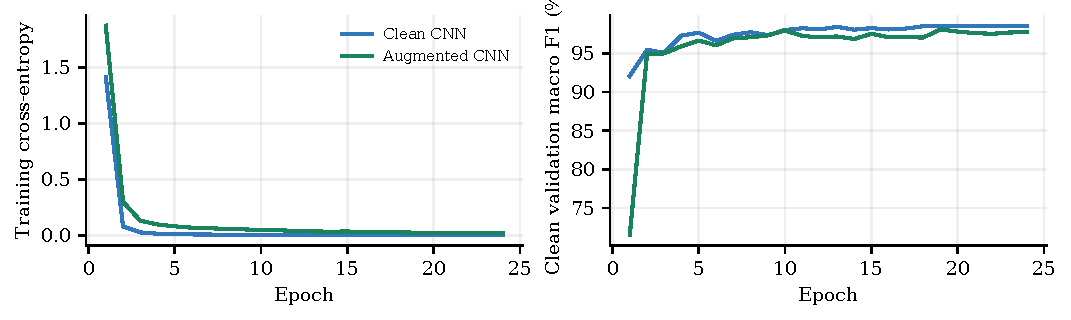
\includegraphics[width=.98\textwidth]{training.pdf}
\caption{CNN training loss and clean validation macro F1. Augmented training loss is measured on transformed inputs, so its absolute value is not directly comparable with the clean model's loss. Checkpoint selection uses the same clean validation criterion for both.}\label{fig:training}
\end{figure*}

Feature extraction uses scikit-image~\cite{skimage}, and feature standardization and linear classification use scikit-learn~\cite{sklearn}. The remainder of the training and evaluation pipeline is implemented in the accompanying project source.

\begin{figure*}[t]\centering
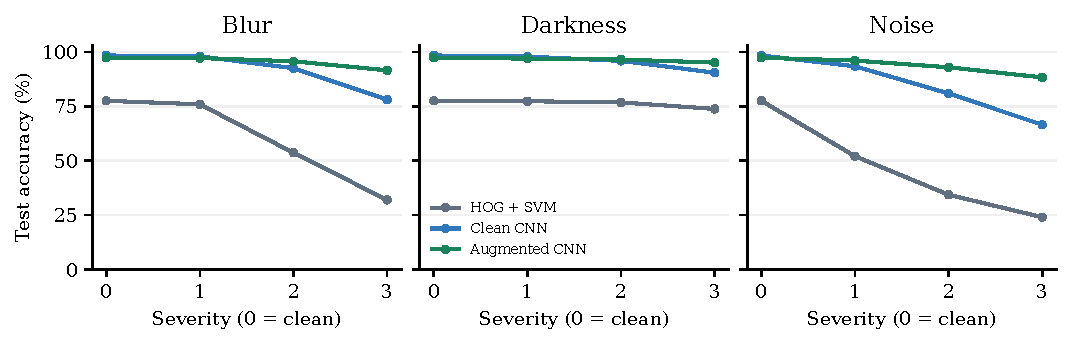
\includegraphics[width=.98\textwidth]{robustness.pdf}
\caption{Accuracy on the complete official test set as a function of corruption severity. Level 0 repeats each model's clean accuracy. Distortion parameters are defined in Table~\ref{tab:conditions}; the horizontal scale is ordinal and is not a shared physical unit across panels.}\label{fig:robustness}
\end{figure*}

\begin{figure*}[t]\centering
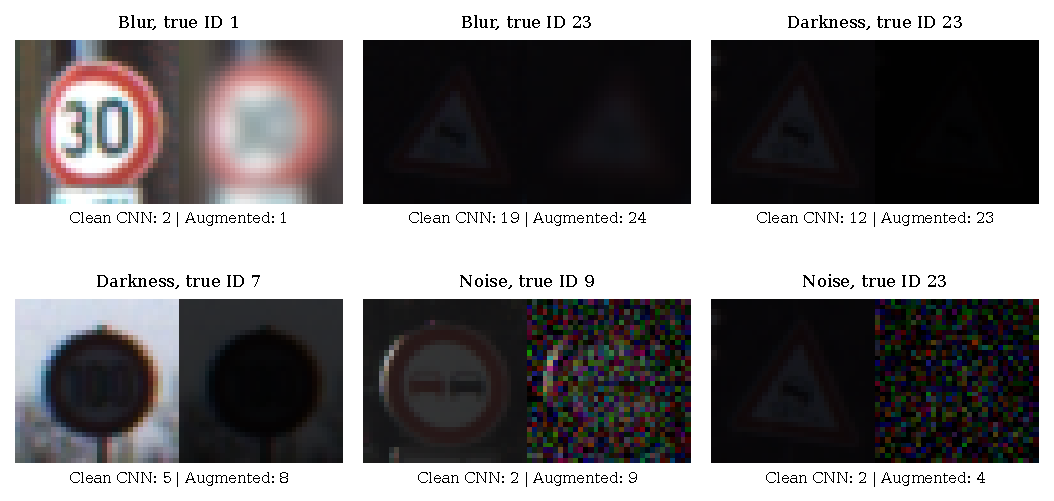
\includegraphics[width=.95\textwidth]{examples.pdf}
\caption{Deterministic qualitative examples. Each tile shows the original crop on the left and a severity-3 version on the right. For each corruption, one augmentation recovery and one remaining augmented-model error are selected by first test-set index. Predictions below each tile refer to the distorted image. This selection illustrates behavior and is not a random estimate of typical performance.}\label{fig:examples}
\end{figure*}

\section{Results and Analysis}
\subsection{Original Test Images}
Table~\ref{tab:overall} summarizes clean and corrupted performance. The clean CNN reaches 98.38\% accuracy and 97.75\% macro F1. The augmented CNN reaches 97.33\% accuracy and 95.87\% macro F1. Their clean-accuracy difference, augmented minus clean, is -1.05 percentage points. HOG--SVM obtains 77.55\% clean accuracy. These results compare models under the specified resizing, features, and training budget; they do not reproduce GTSRB competition submissions.

\begin{table}[t]\centering
\caption{Official-test results (\%). Corrupted metrics average nine conditions; each condition contains 12,630 images.}\label{tab:overall}
\begin{tabular}{lrrrr}\toprule
& \multicolumn{2}{c}{Clean} & \multicolumn{2}{c}{Corrupted mean}\\
Model & Acc. & Macro F1 & Acc. & Macro F1\\\midrule
HOG--SVM & 77.55 & 71.44 & 55.55 & 49.75\\
Clean CNN & 98.38 & 97.75 & 88.18 & 85.33\\
Aug. CNN & 97.33 & 95.87 & 94.47 & 92.38\\\bottomrule
\end{tabular}\end{table}

\subsection{Response to Image Degradation}
Figure~\ref{fig:robustness} plots accuracy as severity increases. Table~\ref{tab:severe} gives the strongest tested conditions. The augmented CNN's mean corrupted accuracy changes by +6.29 percentage points relative to the clean CNN. This is the central measured effect of corruption exposure in the present configuration. It is an average over selected transformations, so the per-condition results are necessary to determine where that aggregate effect comes from.



\begin{table}[t]\centering
\caption{Accuracy (\%) at severity 3, the strongest tested condition for each corruption.}\label{tab:severe}
\begin{tabular}{lrrr}\toprule
Model & Blur & Darkness & Noise\\\midrule
HOG--SVM & 31.97 & 73.81 & 24.03\\
Clean CNN & 78.06 & 90.47 & 66.53\\
Aug. CNN & 91.55 & 95.10 & 88.29\\\bottomrule
\end{tabular}\end{table}

At severity 3 for blur, the clean CNN obtains 78.06\% accuracy and the augmented CNN obtains 91.55\%, a change of +13.49 percentage points. The HOG--SVM baseline reaches 31.97\% under the same transformation.

At severity 3 for darkness, the clean CNN obtains 90.47\% accuracy and the augmented CNN obtains 95.10\%, a change of +4.63 percentage points. The HOG--SVM baseline reaches 73.81\% under the same transformation.

At severity 3 for noise, the clean CNN obtains 66.53\% accuracy and the augmented CNN obtains 88.29\%, a change of +21.76 percentage points. The HOG--SVM baseline reaches 24.03\% under the same transformation.

The HOG descriptor is based on locally normalized gradients and discards color. Brightness scaling can leave gradient orientation relatively stable before quantization, while noise introduces spurious local gradients and blur removes fine spatial structure. CNNs preserve RGB information and learn their representation jointly with classification, but clean training alone does not explicitly penalize mistakes on the synthetic corruptions. Augmented training changes that objective by exposing the model to transformed examples. These are plausible mechanisms for the observed patterns; the experiment does not directly measure internal feature invariance or establish a causal explanation for every class-wise error.

\subsection{Paired Outcomes and Failure Analysis}
Table~\ref{tab:paired} compares the CNNs image by image at severity 3. ``Aug. only'' counts images correctly classified only by the augmented network, while ``clean only'' counts the reverse. Their difference exactly determines the net change in the number of correct predictions for that condition. These descriptive counts make clear that an aggregate improvement need not mean every individual prediction improves.

\begin{table}[t]\centering
\caption{Paired CNN outcomes on severity-3 images. Each row sums to 12,630.}\label{tab:paired}
\begin{tabular}{lrrrr}\toprule
& Both & Aug. & Clean & Both\\
Condition & correct & only & only & wrong\\\midrule
Blur & 9,700 & 1,863 & 159 & 908 \\
Darkness & 11,256 & 755 & 170 & 449 \\
Noise & 8,175 & 2,976 & 228 & 1,251 \\
\bottomrule\end{tabular}\end{table}



Figure~\ref{fig:examples} shows both recoveries and failures, with an explicit selection rule to avoid presenting only favorable cases. Under severe blur, visually similar signs can lose the details that distinguish their class. Under darkness and noise, clipping and 8-bit quantization can remove information that training cannot restore. A confident softmax output can still be wrong; probabilities in the demo have not been calibrated and should not be interpreted as a safety guarantee.

For the augmented CNN on original images, the largest off-diagonal confusion is true class 7 (Speed limit (100km/h)) predicted as class 8 (Speed limit (120km/h)), with 31 images. The exported per-class CSV contains category support and accuracy for every model, and Fig.~\ref{fig:perclass} shows the distribution across all 43 IDs. Rare-category scores can change substantially with a small number of mistakes. Reporting macro F1 alongside overall accuracy helps expose this issue, although it does not remove sampling uncertainty.

\begin{figure}[t]\centering
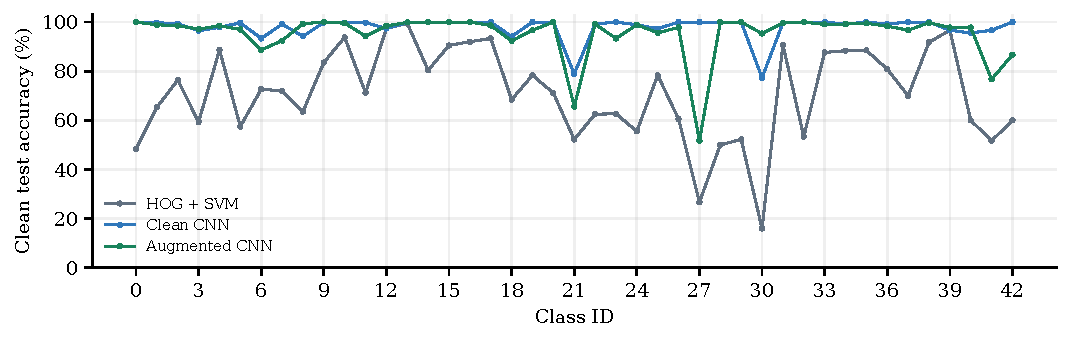
\includegraphics[width=\columnwidth]{per_class.pdf}
\caption{Clean accuracy for each category. Numeric class IDs map to the supplied sign-name file. All classes are included; the axis labels are subsampled for readability.}\label{fig:perclass}
\end{figure}

\subsection{Limitations and Reproducibility}
The training and validation split is track-disjoint, but the supplied official test filenames do not expose physical-sign groups. No track-level uncertainty interval is therefore reported for the test results. A single seed also leaves initialization variance unquantified. Broader evidence would require repeated runs and evaluation on an independently collected dataset or corruption families not represented during training.

The comparison does not isolate every architectural factor: HOG uses grayscale while CNNs use RGB, the SVM is linear, and only one hyperparameter configuration is evaluated. The CNN ablation is more controlled because architecture and fitting settings are held fixed. Its augmentation covers the same three corruption families used for evaluation, so the findings demonstrate robustness within those selected families rather than general robustness to arbitrary distribution shifts. The training and test transformations share severity ranges but use different samples and independent source images.

The reproducibility package records CSV hashes, code hashes, package versions, hardware, split membership, epoch histories, saved checkpoints, raw predicted classes for all ten conditions, clean CNN probabilities, and aggregate metrics. CUDA deterministic convolution settings and fixed seeds reduce variability, but exact numerical identity is not guaranteed across drivers, GPUs, or library versions. The provided local demo applies the same resizing and evaluation transformations as the experiment. It can classify the included examples without access to the full dataset after models are trained.

\balance
\section{Conclusion}
This project implemented a complete cropped-sign recognition and robustness pipeline, connecting image preprocessing, engineered features, linear classification, convolutional representation learning, and controlled experimentation. Under the measured setup, the clean-trained and augmented CNNs achieve 98.38\% and 97.33\% clean accuracy, and 88.18\% and 94.47\% mean corrupted accuracy. The difference of +6.29 percentage points in mean corrupted accuracy describes the observed effect of the training intervention.

The main lesson is that recognition quality depends on both the representation and the image conditions represented during training. Aggregate clean accuracy should be accompanied by class-wise and corruption-specific evaluation. Future work could add repeated-seed experiments, stronger classical baselines, calibrated uncertainty, and independent real-world degradations before extending the system to detection or video.

\begin{thebibliography}{00}
\bibitem{gtsrb} J. Stallkamp, M. Schlipsing, J. Salmen, and C. Igel, ``Man vs. computer: Benchmarking machine learning algorithms for traffic sign recognition,'' \emph{Neural Networks}, vol. 32, pp. 323--332, 2012, doi: 10.1016/j.neunet.2012.02.016.
\bibitem{hog} N. Dalal and B. Triggs, ``Histograms of oriented gradients for human detection,'' in \emph{Proc. IEEE CVPR}, vol. 1, 2005, pp. 886--893, doi: 10.1109/CVPR.2005.177.
\bibitem{corruption} D. Hendrycks and T. Dietterich, ``Benchmarking neural network robustness to common corruptions and perturbations,'' in \emph{Proc. ICLR}, 2019. [Online]. Available: \url{https://arxiv.org/abs/1903.12261}
\bibitem{adamw} I. Loshchilov and F. Hutter, ``Decoupled weight decay regularization,'' in \emph{Proc. ICLR}, 2019. [Online]. Available: \url{https://arxiv.org/abs/1711.05101}
\bibitem{sklearn} F. Pedregosa \emph{et al.}, ``Scikit-learn: Machine learning in Python,'' \emph{J. Mach. Learn. Res.}, vol. 12, pp. 2825--2830, 2011. [Online]. Available: \url{https://jmlr.org/papers/v12/pedregosa11a.html}
\bibitem{skimage} S. van der Walt \emph{et al.}, ``Scikit-image: Image processing in Python,'' \emph{PeerJ}, vol. 2, e453, 2014, doi: 10.7717/peerj.453.
\bibitem{augmix} D. Hendrycks, N. Mu, E. D. Cubuk, B. Zoph, J. Gilmer, and B. Lakshminarayanan, ``AugMix: A simple data processing method to improve robustness and uncertainty,'' in \emph{Proc. ICLR}, 2020. [Online]. Available: \url{https://arxiv.org/abs/1912.02781}
\bibitem{dinov3} O. Sim\'eoni \emph{et al.}, ``DINOv3,'' arXiv:2508.10104, 2025. [Online]. Available: \url{https://arxiv.org/abs/2508.10104}
\end{thebibliography}
\end{document}
